% 1.9. Sử dụng hàm đơn điệu
\begin{frame}{1.9 SỬ DỤNG HÀM ĐƠN ĐIỆU\hspace{2cm}  73. Nguyễn Thị Hà Thương} 
%\framesubtitle{} 
\begin{block}{\textbf{Định lí}}
Cho hàm số $y=f(x)$ xác định, liên tục trong khoảng $(a;b)$. Khi đó:\\
\begin{itemize}
    \item Nếu $f'(x)>0 \quad \forall x \in (a;b)$ thì $f(x)$ đồng biến trên khoảng $(a;b)$.
    \item Nếu $f'(x)<0 \quad \forall x \in (a;b)$ thì $f(x)$ nghịch biến trên khoảng $(a;b)$.
\end{itemize}
    
\end{block} 
\pause
\textbf{Nhận xét.}\\
Việc chứng minh $A \geq B$ được đưa về xét hàm $A-B$ qua đạo hàm.\\
$\rightarrow$ \text{Từ tính đồng biến hay nghịch biến của $A-B$ ta suy ra bất đẳng thức.}
\end{frame} 

\begin{frame}{1.9 SỬ DỤNG HÀM ĐƠN ĐIỆU\hspace{2cm}  73. Nguyễn Thị Hà Thương} 
%\framesubtitle{} 
\begin{block}{Ví dụ}
Chứng minh: $sinx<x<tanx, \forall x\in (0;\frac{\pi}{2})$
\end{block}
\pause

Xét hàm số $f(x)=sinx-x$ trên khoảng $(0;\frac{\pi}{2})$\\
$f'(x)=cosx-1 < 0$ $\Rightarrow$ {$f(x)$ \quad \text{nghịch biến}}\\
$0<x<\frac{\pi}{2}$ $\Rightarrow$ {$f(0) > f(x)$} \quad $\Rightarrow${$0 > sinx - x$}\quad hay \quad $x > sinx$ \quad $(1)$\\
\pause
Xét hàm số $g(x)=tanx-x$ trên khoảng $(0;\frac{\pi}{2})$\\
$g'(x)=\frac{1}{cos^2x}-1=\frac{1-cos^2x}{cos^2x} > 0$ $\Rightarrow${$g(x)$ \quad \text{đồng biến}}\\
$0<x<\frac{\pi}{2}$ $\Rightarrow${$g(0) < g(x)$} \quad $\Rightarrow${$0 < tanx - x$}\quad hay \quad $x < tanx$ \quad $(2)$\\

\indent Từ $(1)$ và $(2)$ $\Rightarrow${\text{đpcm}}
\end{frame} 

\begin{frame}{1.9 SỬ DỤNG HÀM ĐƠN ĐIỆU\hspace{2cm}  73. Nguyễn Thị Hà Thương} 
%\framesubtitle{} 
\begin{block}{\textbf{Bài tập đề xuất}}
\large Cho $n\in\mathbb{N}^*$, chứng minh:\\
\centering \large $\frac{1}{\sqrt{1^2+1}}+\frac{1}{\sqrt{2^2+2}}+...+\frac{1}{\sqrt{n^2+n}}>\ln{(n+1)}$
\end{block}

\pause
\large Xét hàm số $f(x)=\frac{1}{\sqrt{x^2+x}}-\ln{(x+1)}+\ln{x}, \forall x \geq 1$
\end{frame} 

\begin{frame}{1.9 SỬ DỤNG HÀM ĐƠN ĐIỆU\hspace{2cm}  73. Nguyễn Thị Hà Thương} 
%\framesubtitle{}
\large $f(x)=\frac{1}{\sqrt{x^2+x}}-\ln{(x+1)}+\ln{x}, \forall x \geq 1$\\
\large $f'(x)= \frac{\frac{-2x-1}{2\sqrt{x^2+x}}}{x^2+x} - \frac{1}{x+1} + \frac{1}{x} = \frac{2\sqrt{x^2+x}-2x-1}{2(x^2+x)\sqrt{x^2+x}} < 0, \forall x \geq 1 $
\pause
\begin{center}
    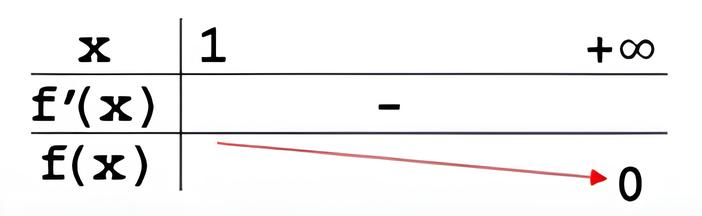
\includegraphics[scale=0.2]{bbt (1.9).JPG}
\end{center}
\pause
\large Suy ra $f(x)>0,\forall x \geq 1 $\\
\large nên $\frac{1}{\sqrt{x^2+x}} > \ln{(x+1)} - \ln{x}$
\end{frame}

\begin{frame}{1.9 SỬ DỤNG HÀM ĐƠN ĐIỆU\hspace{2cm}  73. Nguyễn Thị Hà Thương} 
	%\framesubtitle{}
		Do $\frac{1}{\sqrt{x^2+x}} > \ln{(x+1)} - \ln{x}$, ta có:\\
		$\frac{1}{\sqrt{1^2+1}} > \ln{2} - \ln{1}$\\
		$\frac{1}{\sqrt{2^2+2}} > \ln{3} - \ln{2}$\\
		...\\
		$\frac{1}{\sqrt{n^2+n}} > \ln{(n+1)} - \ln{n}$\\
$\Rightarrow$ $\frac{1}{\sqrt{1^2+1}}+\frac{1}{\sqrt{2^2+2}}+...+\frac{1}{\sqrt{n^2+n}} > \ln{(n+1)} - \ln{1} = \ln{(n+1)}$ $\Rightarrow$ {\text{đpcm.}}
\end{frame}

\begin{frame}{1.9 SỬ DỤNG HÀM ĐƠN ĐIỆU\hspace{2cm}  73. Nguyễn Thị Hà Thương}
\begin{block}{\textbf{Bài tập tham khảo} (Thi HSG Quốc gia 1992)}
Chứng minh rằng, với mọi số tự nhiên $n>1$ ta có:\\
\centering $\sqrt[n]{1+\frac{\sqrt[n]{n}}{n}}+\sqrt[n]{1-\frac{\sqrt[n]{n}}{n}} < 2$
\end{block}
\pause
Đặt $x=\frac{\sqrt[n]{n}}{n} \in (0;1)$. Bất đẳng thức cần chứng minh trở thành:\\
\begin{center}
$\sqrt[n]{1+x}+\sqrt[n]{1-x} < 2, \forall x\in (0;1)$.
\end{center}
\pause
Xét hàm số $f(x)=\sqrt[n]{1+x}+\sqrt[n]{1-x}$ liên tục trên khoảng $(0;1)$ có:\\
$f'(x)= \frac{1}{n}(\frac{1}{\sqrt[n]{(1+x)^{n-1}}}-\frac{1}{\sqrt[n]{(1-x)^{n-1}}})<0, \forall x \in (0;1)$\\
Vậy $f(x)$ nghịch biến trên $(0;1)$ nên $f(x)<f(0)=2 \Rightarrow \text{đpcm}$
\end{frame}

